\usepackage[utf8]{inputenc}
\usepackage[T1]{fontenc}
\usepackage{mathptmx}
\usepackage[scaled=.90]{helvet}
\usepackage{courier}
\usepackage{caption}
\captionsetup{labelformat=empty,labelsep=none}
\usepackage{verbatim}
\usepackage{hyperref}
\usepackage{listings}
% strikethrough (\sout)
\usepackage{ulem}
\lstset{language=Perl,basicstyle=\normalsize,tabsize=3,showstringspaces=false}

\title{Monitoring with Nagios and Check\_MK}
\author[racke]{Stefan Hornburg (Racke)\\ \texttt{racke@linuxia.de}}
\date{DORS/CLUC 2015, Zagreb}

\begin{document}
\maketitle{}

\begin{frame}
  \titlepage
\end{frame}

\tableofcontents

% Introduction
% Why I'm talking about this subject?

\section{Monitoring}

\begin{frame}[fragile]{Monitoring}

\begin{itemize}
\item Why ?
\item Who ?
\item What ?
\end{itemize}
\end{frame}

\subsection{Why ?}

Availability of a server usually means he can be reached with a PING.

If you depend on services from other parties, you can assume that
they are monitoring them itself. But can you always rely on that?

\begin{frame}[fragile]{Why ?}
\begin{itemize}
\item Availability of servers and services
\item 3rd party services (SLA)
\end{itemize}
\end{frame}

\begin{frame}[fragile]{Who ?}
\begin{itemize}
\item Companies
\item Open Source Projects
\end{itemize}
\end{frame}

% \subsection{Use Cases}
% \begin{frame}[fragile]{Use Cases}
% \begin{itemize}
% \item Inventory
% \item Backup
% \end{itemize}
% \end{frame}

What should be monitored? Aside from standard checks, there are 
lot of other things you might want to check which aren't obvious.
I'm going through to an use case of a mailserver and give you
a couple of examples for custom checks.

\subsection{Use Case Mailserver}
Early in my career as freelancer I worked on a setup for an ISP
in Zurich, Switzerland. We designed the firewall, web servers
and mail server on our own. 

Back then, it was a much more easy job to do
so, literally no SPAM and Virus. Also monitoring started much
later.

\subsubsection{Basic Checks}

First a few examples on basic checks applied to all servers.

Disk can be eaten up slowly by incoming emails or rather
quickly by runaway applications filling log files.

\begin{frame}{Basic Checks}
\begin{itemize}
\item CPU
\item Memory Usage
\item TCP Connections
\item Disk Usage
\end{itemize}
\end{frame}

\subsubsection{Email Checks}

\begin{frame}{Email Checks I}

% IMAP: max connections (multiple per client)

\begin{itemize}
\item SMTP
\item IMAP/POP
\item Webmail
\item Database
\end{itemize}
\end{frame}

\begin{frame}{Email Checks II}
\begin{itemize}
\item Virenscanner
\item Spamfilter
\end{itemize}
\end{frame}

\begin{frame}{Email Checks III}
% newsletter
% something is going wrong
% PHP worm
\begin{itemize}
\item Queue
\end{itemize}
\end{frame}

\begin{frame}{Email Checks IV}
\begin{itemize}
\item Blacklists
\end{itemize}
\end{frame}

\subsection{More Checks}

Backups are very important and you really need to make sure
that they are done and can be restored properly.

\begin{frame}[fragile]{More Checks}

\begin{itemize}
\item stuck jobs
\item products on Amazon
\item orders
\item crashes
\item import files
\item backups
\item MySQL replication
\end{itemize}
\end{frame}

\section{Nagios}

\begin{frame}[fragile]{Nagios}
\begin{itemize}
\item Advantages
\item Checks
\item Disadvantages
\end{itemize}
\end{frame}

\subsection{Advantages}
\begin{frame}[fragile]{Advantages}
\begin{itemize}
\item Flexible
\item Plugins (simple model)
\item Community
\item Ecosystem
\end{itemize}
\end{frame}

\subsection{Checks}
All checks in Nagios are realized by plugins.

We distinguish between active and passive checks.

Active checks are initiated by Nagios itself,
while passive checks are performed and submitted
to Nagios.

\begin{frame}[fragile]{Checks}
\begin{itemize}
\item Check = Plugin
\verb|/usr/lib/nagios/plugins/check_http|
\end{itemize}

\begin{itemize}
\item active checks
\item passive checks
\end{itemize}

\end{frame}

\subsubsection{Check States}

Each of these checks results in one of the four
following states:

\begin{frame}[fragile]{Check States}

\begin{itemize}
\item OK
\item WARNING 
\item CRITICAL
\item UNKNOWN
\end{itemize}
\end{frame}

UNKNOWN - misconfiguration

\begin{frame}[fragile]{Text and Performance Data}
\begin{lstlisting}
HTTP OK: HTTP/1.1 200 OK -
33920 bytes in 0.263 second response time

time=0.262644s;;;0.000000 size=33920B;;;0
\end{lstlisting}
\end{frame}

\begin{frame}{Performance Graph}
\begin{figure}
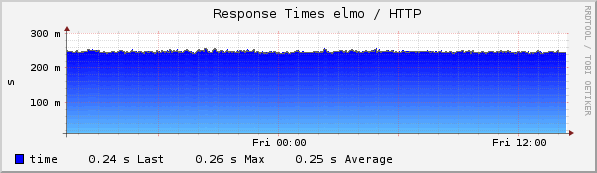
\includegraphics[width=\textwidth]{images/perfdata.png}
\end{figure}
\end{frame}

\subsection{Concerns}

The German Linux Magazin did a recent survey amongst users
who checked alternatives for out-of-the-box Nagios.

The main two concerns are raised in environments with lots
of servers.

The first one is complicated configuration of big text files
and the other is the scalability.

\begin{frame}{Concerns}

\begin{itemize}
\item Configuration
\item Scalability in large environments
\end{itemize}
\end{frame}

\section{Check\_MK}

What is check\_mk? Nagios add-on.

\begin{frame}[fragile]{Check\_MK}
\begin{itemize}
\item Features
\item Components
\item Installation \& Configuration
\item Practical Advice
\end{itemize}
\end{frame}

\subsection{Features}

Which features adds \verb|Check_MK| to a standard Nagios installation?

\begin{frame}[fragile]{Features}
\begin{itemize}
\item Automatic service detection
\item Rule based, hierarchical confirmation
\item High performance through passive checks
\item Creates Nagios configs for you
\end{itemize}
\end{frame}

\subsection{Components}
% Source: Check_MK homepage

Configuration and check engine:

automatic servic recognition
configuration generator

Livestatus
quick and efficient access to status data

Multisite
distribute monitoring

WATO
Web Administration Tool
management of users, roles, groups, time periods, 
classical Nagios-Checks and much more

Notify:
Notification

Event Console:
processing of SNMP-Traps and log messages

\begin{frame}[fragile]{Components}
\begin{itemize}
\item Configuration \& Check Engine
\item Livestatus
\item Multisite
\item WATO
\item Notify
\item Business Intelligence
\item Mobile
\item Event Console
\end{itemize}
\end{frame}

\begin{frame}{Architecture}
\begin{figure}
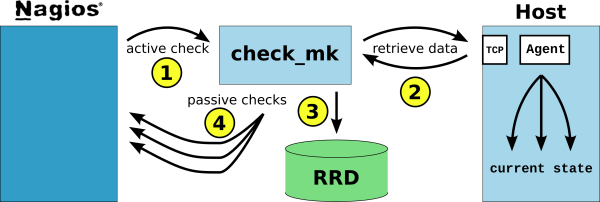
\includegraphics[width=\textwidth]{images/overview_600_trans.png}
\end{figure}
Source: http://mathias-kettner.de/bilder/overview\_600.trans.png
\end{frame}

\subsection{Installation \& Configuration}

\begin{frame}[fragile]{Installation}
\begin{itemize}
\item Open Monitoring Distribution \url{http://omdistro.org/}
\end{itemize}
\end{frame}

\subsubsection{Adding and updating hosts}
There are two ways to add or update hosts, you can do
it through the commandline or with the WATO administration
interface.

check\_mk -I finds new services on the hosts on the commandline.

check\_mk -II finds renews services (and drops old services) 
on the hosts on the commandline.

check\_mk -O rewrites the configuration and reloads Nagios

\begin{frame}[fragile]{Adding and updating hosts}
\begin{description}
\item[Inventory] \verb|check_mk -I linuxia|
\item[Inventory] \verb|check_mk -II linuxia|
\item[Reload] \verb|check_mk -O linuxia|
\end{description}
\end{frame}

% \begin{frame}[fragile]{WATO}
% \begin{lstlisting}
%  you have set-up the sudo environment correctly. e.g. proceed as follows:

% install sudo package
% Append the following to the /etc/sudoers file:
% # Needed for WATO - the Check_MK Web Administration ToolDefaults:www-data !requirettywww-data ALL = (nagios) NOPASSWD: /usr/bin/check_mk --automation *
% Retry this operation
% \end{lstlisting}
% \end{frame}


\subsubsection{Custom Checks}

% RPE = Remote Plugin Executor
% soft migration from NRPE to check_mk
% third party plugins
\begin{frame}[fragile]{Migrating from NRPE to MRPE}
\begin{description}
\item[Configuration file] \verb|/etc/check_mk/mrpe.cfg|
\item[Example] \verb|APT  /usr/lib/nagios/plugins/check_apt|
\end{description}
\end{frame}

\subsection{Practical Advice}

\section{Slides}

\begin{frame}[fragile]{Resources}
\begin{description}
\item[Check\_MK Homepage] \url{http://mathias-kettner.com/check_mk.html}
\end{description}
\end{frame}

\begin{frame}{Slides}
Slides:
\url{http://www.linuxia.de/talks/dorscluc2015/nagios-en-beamer.pdf}
\end{frame}

\end{document}

%%% Local Variables: 
%%% mode: latex
%%% TeX-master: t
%%% End: 
